%!TEX root = ../thesis.tex
\chapter{The modulus as activation function} \label{ch:modulus}

\section{Overview}
The idea of decreasing the size of neural networks has been studied since long time ago \autocite{lecun1989, hassibi1993, frankleC19}. Many applications may require to be efficient at training or at inference times, especially the models that need to be executed on mobile and embedded devices \autocite{ooko2021, zapico2021}. One of the most impressive examples is the wake word detection system of the \textit{Google} assistant, which was reported to weight only 14 kilobytes in size \autocite{warden2020}. 

The subfield of machine learning that researches how to minimize the computational cost is commonly known as \textit{TinyML} \autocite{han2022}. \textit{TinyML} not only brings obvious energy consumption benefits but it can also be used to reduce the latency of the response of such systems because the devices would no longer need to query large cloud servers, removing the dependency on internet connections and allowing them to work offline. Furthermore, the common privacy concerns of machine learning applications \autocite{ha2019} can be easily diluted if all the sensible data collected are processed solely into the device, and never leaves home.

This chapter introduces a new non-monotonic activation function --the \textit{modulus}-- which simplicity makes it specially suitable for \textit{TinyML} and other low resource applications: the modulus and its derivative are simply bit-size operations. Interestingly, the gradient norm does not depend on the input, which removes some of the problems reported on other nonlinearities \autocite{lu2020, pascanu13, hochreiter1998, Hochreiter2001}. The experiment results provide evidence that when using the \textit{modulus} activation function on computer vision tasks the models generalize better than with other nonlinearities - up to a 15\% accuracy increase in \textit{CIFAR100} dataset and 4\% in \textit{CIFAR10} dataset (with respect to the benchmark activations tested). 



The code used along this work has been made available in a public repository\footnote{\url{https://github.com/ivallesp/abs}}.


\section{Introduction}
As discussed in section \ref{sec:mlp}, the core piece of all deep learning models is the activation function. They enable the models to produce non-linear abstract representations when applying linear transformations in cascade \autocite{Goodfellow2016}. The most common choice in modern deep learning models is the Rectified Linear Unit (\textit{ReLU}) \autocite{nair2010}. Among other advantages, \textit{ReLU} nonlinearities allow to train deeper neural networks \autocite{xu2015}.

\section{Previous work}
Apart from the \textit{ReLU} in the last years there have appeared many alternative activation functions. The following studies represent some of the most popular examples: \textit{Leaky-ReLU} and \textit{PR-ReLU} \autocite{xu2015}, \textit{ELU} \autocite{djork2016}, \textit{Swish} \autocite{ramachandran2018}, \textit{SELU} \autocite{klambauer2017}, \textit{F/PFLU} \autocite{zhu2020}, \textit{RSigElu} \autocite{Kilicarslan2021} etc. All those activation functions have the following properties in common: nonlinearity, continuity, differentiability and low computational cost (being \textit{Swish} the most computationally expensive option). The majority of the activation functions are monotonic, \textit{Swish} \autocite{ramachandran2018}, \textit{GELU} \autocite{hendrycks2016},  \textit{S-ReLU} \autocite{Jin2016} and \textit{Mish} \autocite{misra2019mish} are some of the most popular modern exceptions. Despite the large pool of alternatives, \textit{ReLU} still appears as the default choice in many applications due to its simplicity and low computational cost \autocite{nair2010}.

This chapter delves into the world of the non-monotonic nonlinearities and proposes the \textit{modulus} function (aka absolute value) as an activation function, providing empirical evidences  proving that this activation function allows deep learning models to converge to better solutions in \textit{CIFAR10}, \textit{CIFAR100} and \textit{MNIST} datasets. 

Compared with other modern non-monotonic nonlinearities such as \textit{Mish} \autocite{misra2019mish}, \textit{PFLU} and \textit{FPFLU} \autocite{zhu2020} or \textit{Swish}  \autocite{ramachandran2018}, the \textit{modulus} has a very low computational cost (equivalent to \textit{ReLU}). This property makes the \textit{modulus} specially useful for \textit{TinyML} \autocite{sanchez2020} and hardware \autocite{Misra2010} applications.

%The contributions of this work are: (1) proposal of the modulus as activation function, (2) the proposed function empirically shows significantly superior results in 75\% of our experiments, (3) we- contribute to the new trend of non-monotonic activation functions with another example showing results in the same direction, (4) the simplicity of the modulus activation function makes it very suitable for hardware applications and \textit{TinyML}, and (5) we- propose two smooth approximation to the \textit{modulus} function, one of them achieving even superior results than the original \textit{modulus}.

%This chapter is organized as follows. Section \ref{sec:modulus_methods} describes the proposed activation function and the ones used for benchmarking. Section \ref{sec:modulus_experiments} describes the experiments conducted and the results achieved. Finally, we- summarize our contribution in section \ref{sec:modulus_conclusions}, enumerating the main conclusions.


% Ideas
% Non-dying regions

\section{Methods} \label{sec:modulus_methods}
\subsection{Modulus activation function}
This section introduces the proposed activation function, the \textit{modulus}: $f(x)=|x|$. This nonlinearity is a continuous, piecewise-linear function consisting of an identity mapping for positive values of $x$, and a negative identity mapping for negative values of $x$. Its derivative (defined below) as well as the modulus function itself, are bit-size operations. This is extremely useful for hardware implementations. Besides, the modulus function can be expressed as $f(x) = \text{sgn}(x)\cdot x$, where $f'(x) = \text{sgn}(x)$. In practice, this means that the derivative can be calculated as part of the forward pass and cached for the \textit{backpropagation}, reducing the total computation. This form is also specially useful in hardware implementations, given that the whole activation function is fully represented as a bit-size operation (the sign function).

$$
f'(x)= \left\{ \begin{array}{lcc}
1 &   \text{if}  & x > 0 \\
-1 &  \text{if} & x < 0
\end{array} \right.
$$

Notice that the \textit{modulus} function is differentiable everywhere except in $x = 0$. For practical purposes,  $f'(0) := 1$  so that the derivative is defined for all the range of $x$ values, similar to the case of \textit{ReLU} \autocite{Goodfellow2016}. See figure \ref{fig:activations}h for a graphical representation.


The \textit{modulus} activation function belongs, in essence, to the family of rectifier functions \autocite{glorot2015} . In fact, it is equivalent to a \textit{Leaky-ReLU} with $\alpha=-1$. However \textit{Leaky-ReLU} was originally defined to take values of alpha strictly higher than 0 \autocite{xu2015}. Furthermore, \textit{modulus} achieves significantly superior results than the \textit{Leaky-ReLU}.

\begin{figure}[h!]
	\centering
	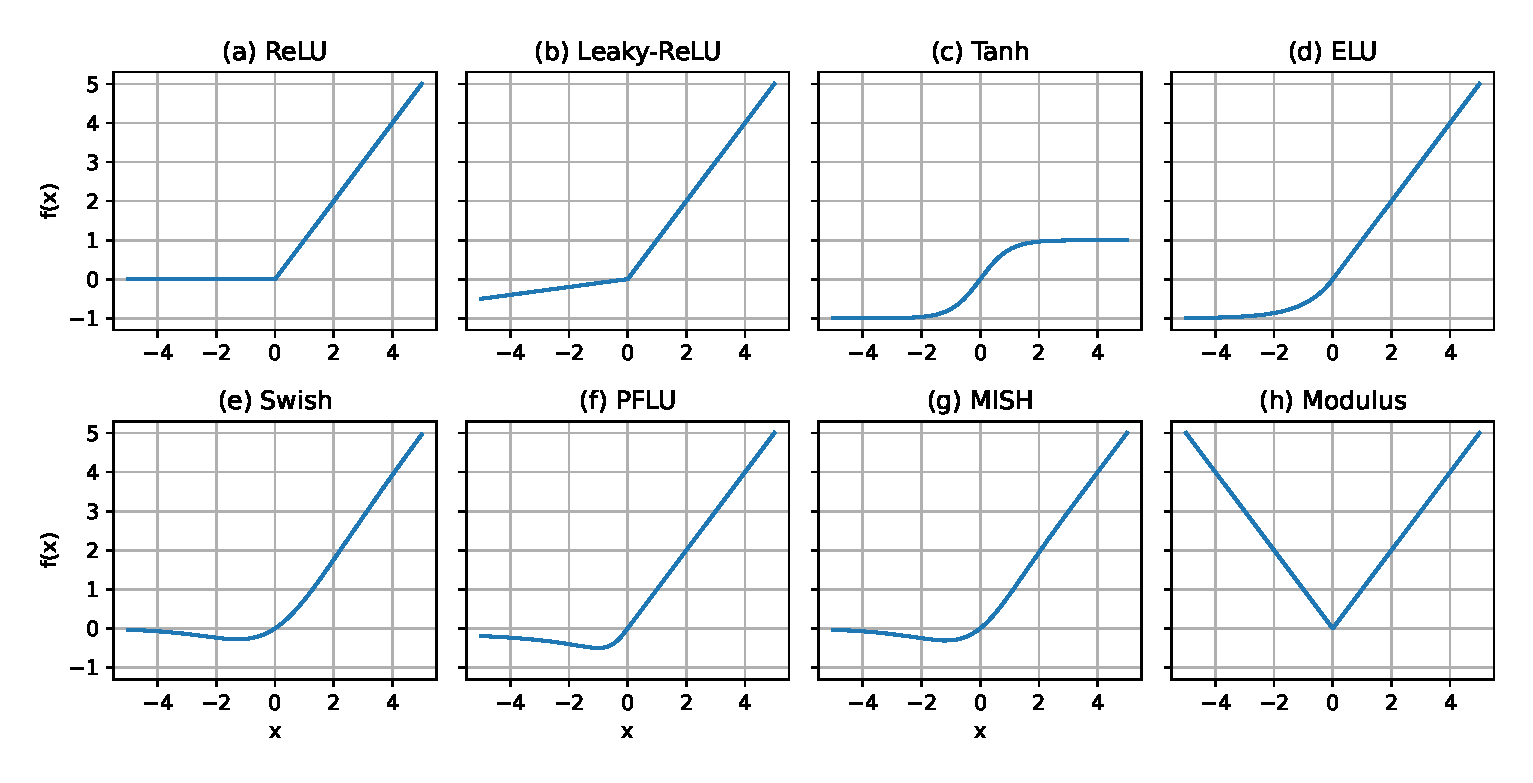
\includegraphics[width=1.0\linewidth]{modulus/images/activations}
	\caption{Nonlinearities used along this study. (a-g) are benchmark activation functions that showed good performance in previous studies. (h) is the \textit{modulus} activation function proposed in this chapter. For this example, the default hyper-parameters have been used for the \textit{Leaky-ReLU}, \textit{ELU} and \textit{Swish} activation functions, respectively.
	}
	\label{fig:activations}
\end{figure}

The benefit of this activation function with respect to the other rectifiers is that the norm of its gradient is constant ($||\nabla_x f|| = 1 \quad \forall x$) and hence it does not depend on the input value. This property is desirable when optimizing the parameters of a neural network with gradient descent algorithms, as there are no input values for which the neuron saturates \autocite{glorot2010} (i.e. values of x for which the gradient of the activation function is close to zero). This naturally removes the dying neurons \autocite{lu2020} and vanishing gradient problems \autocite{pascanu13, hochreiter1998, Hochreiter2001}.

\subsection{Smooth approximations of the modulus function}
The \textit{modulus} function is not differentiable when $x=0$. To study if this property harms the performance of the models in any way, two alternative smooth approximations of the \textit{modulus} function have been tested as an additional experiment. See figure \ref{fig:activationssmooth} for a visual representation. The two approximations are defined below.


\begin{figure}[h!]
	\centering
	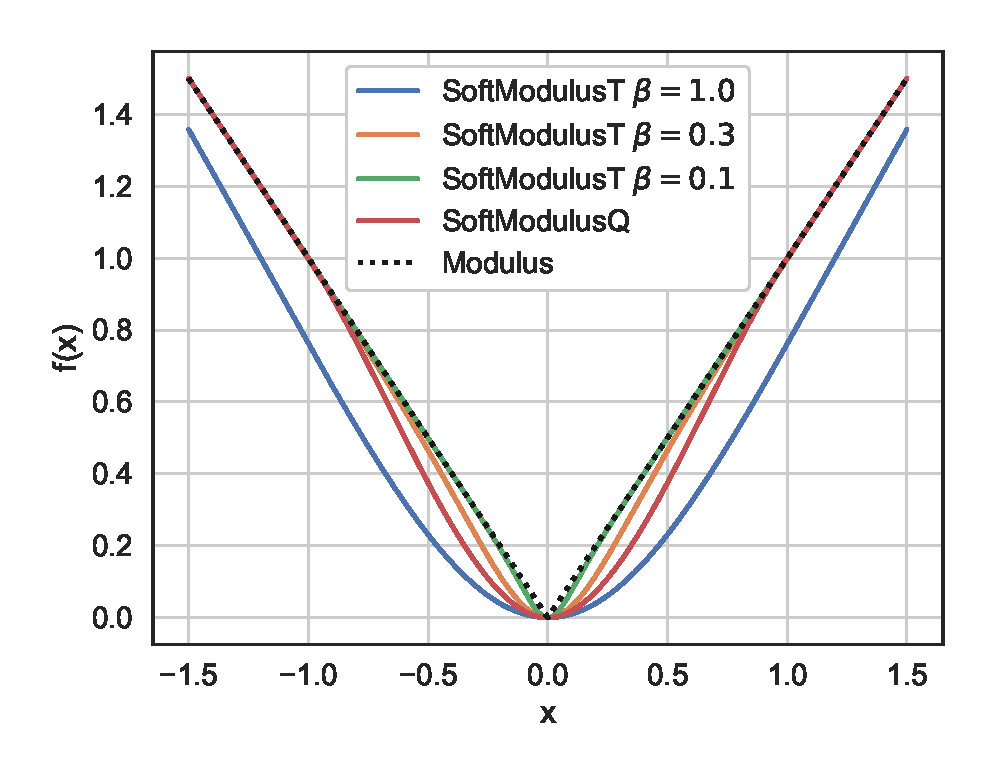
\includegraphics[width=0.5\linewidth]{modulus/images/activations_smooth}
	\caption{Representation of the two \textit{SoftModulus} activation functions compared with the original \textit{modulus}: \textit{SoftModulusQ} and \textit{SoftModulusT}.}
	\label{fig:activationssmooth}
\end{figure}


\subsubsection{Quadratic approximation}
A fuzzy set approach is chosen as a method to combine the modulus function with a quadratic function (see figure \ref{fig:fuzzy_funcs}) to get a smooth approximation. For that, three membership functions are defined in figure \ref{fig:fuzzy} and equations \ref{eq:mulow}, \ref{eq:mumid}, \ref{eq:muhigh}.

\begin{figure}[h!]
	\centering
	\includegraphics[width=0.7\linewidth]{modulus/images/funcs_quad}
	\caption{Quadratic and modulus functions, together with the combined one (in blue, red and green, respectively).}
	\label{fig:fuzzy_funcs}
\end{figure}

\begin{figure}[h!]
	\centering
	\includegraphics[width=0.7\linewidth]{modulus/images/fuzzy}
	\caption{Membership functions used to combine the quadratic and modulus functions.)}
	\label{fig:fuzzy}
\end{figure}

\begin{equation}
\label{eq:mulow}
\mu^x_{\text{low}}= \left\{ \begin{array}{lcc}
1 &   \text{if}  & x < -1 \\
-x & \text{if}  & -1 \leq x < 0 \\
0 &  \text{if} & x \geq 0
\end{array}
\right.
\end{equation}

\begin{equation}
\label{eq:mumid}
\mu^x_{\text{med}}= \left\{ \begin{array}{lcc}
0 &   \text{if}  & x < -1 \\
x+1 & \text{if}  & -1 \leq x < 0 \\
1-x & \text{if}  & 0 \leq x < 1 \\
0 &  \text{if} & x \geq 1
\end{array}
\right.
\end{equation}

\begin{equation}
\label{eq:muhigh}
\mu^x_{\text{high}}= \left\{ \begin{array}{lcc}
0 &   \text{if}  & x < 0 \\
x & \text{if}  & 0 \leq x < 1 \\
1 &  \text{if} & x \geq 1
\end{array}
\right.
\end{equation}

Let $f^x_{\text{low}}=-x$, $f^x_{\text{med}}=x^2$ and $f^x_{\text{high}}=x$. These functions are combined with the membership functions to get the quadratic approximation.

\begin{itemize}
	\item For $x < -1$:  $\hat{f}(x)=\frac{f^x_{\text{low}} \cdot \mu^x_{\text{low}}}{\mu^x_{\text{low}}}=-x$

	\item For $-1\leq x < 0$:  $\hat{f}(x)=\frac{f^x_{\text{low}} \cdot \mu^x_{\text{low}} + f^x_{\text{med}} \cdot \mu^x_{\text{med}}}{\mu^x_{\text{low}} + \mu^x_{\text{med}}}=\frac{(x+1)x^2+(-x)(-x)}{1+x-x}=x^3 + 2x^2$

	\item For $0\leq x < 1$:  $\hat{f}(x)=\frac{f^x_{\text{med}} \cdot \mu^x_{\text{med}} + f^x_{\text{high}} \cdot \mu^x_{\text{high}}}{\mu^x_{\text{med}} + \mu^x_{\text{high}}}=\frac{(1-x)x^2+x\cdot x}{1-x+x}=-x^3 + 2x^2$

	\item For $x \geq 1$:  $\hat{f}(x)=\frac{f^x_{\text{high}} \cdot \mu^x_{\text{high}}}{\mu^x_{\text{high}}}=x$
\end{itemize}

Combining and simplifying all the above expressions the final activation function is obtained. This approximation is subsequently referred as \textit{SoftModulusQ}.


$$
f(x)= \left\{ \begin{array}{lcc}
x^2 \cdot (2-|x|) &  \text{if} & |x| \leq 1 \\
|x| &   \text{if}  & |x| > 1
\end{array}
\right.
$$


\subsubsection{Hyperbolic tangent approximation}
Starting from the modulus function $f(x)=sgn(x)\cdot x$, the $sgn$ function is approximated as follows $sgn(x) \approx \tanh(x/\beta)$, where $\beta \in [0, 1]$ is a tunable hyperparameter that controls how acute the ``V'' transition is. The smaller the $\beta$, the closest the approximation is to the \textit{modulus}. A value of $\beta=0.01$ is used along all the trained models. In the rest of the chapter, this approximation is referred as \textit{SoftModulusT}.

	$$f(x) = x \cdot \tanh(x/\beta)$$



% TODO: \usepackage{graphicx} required

\subsection{Benchmark activation functions}
The following activation functions have been used as a benchmark to compare the performance of the proposed one.


\begin{itemize}
	\item \textit{Tanh}: the hyperbolic tangent has been one of the most popular choices (together with the \textit{sigmoid}), before \textit{ReLU} was proposed \autocite{lecun2012}. Among many other desirable properties, its derivative is very simple: $(\tanh x)'=1-\tanh^2 x$. This property was very beneficial specially before automatic differentiation tools appeared. Besides, similar to the proposed activation function, the derivative can be easily calculated during forward pass and cached for the backward pass.
	\item \textit{ReLU}: this activation function was published in 2010 as an alternative to train \textit{Restricted Boltzman Machines} \autocite{nair2010}. It is defined as $f(x) = \max(0,x)$. It allowed training deeper neural networks by solving the vanishing gradient problems typically happening with saturating activation functions. As it can be seen in the formula, ReLU outputs zero if the input is negative. This brings sparsity to the non-linear representation, at the cost of potentially finding optimization problems due to the fact that the derivative when $x<0$ is zero (dying neurons, for instance).
	\item \textit{Leaky-ReLU}: the \textit{Leaky-ReLU} \autocite{xu2015} attempted to solve the problem known as \textit{dying neurons} in the \textit{ReLUs} by adding a small linear term in the negative side of $x$: $f(x) = \max(x/\beta, x)$, where $\beta$ is a hyperparameter to be tuned: $\beta>1$ and $\sigma$ is the logistic function.
	\item \textit{ELU}: this is a smooth version of \textit{ReLU} \autocite{djork2016} that approaches asymptotically to -1 when $x=-\inf$. Unlike ReLUs, it is differentiable everywhere and can produce negative values. This activation function is formally defined as follows. $\alpha$ is a tunable hyperparameter.
	$$
	f(x)= \left\{ \begin{array}{lcc}
		x &   \text{if}  & x > 0 \\
 \alpha(e^x - 1) &  \text{if} & x \leq 0
	\end{array}
	\right.
	$$

	\item \textit{Swish}: this is one of the few non-monotonic activation functions formally published \autocite{ramachandran2018}. It is defined as $f(x) = x \cdot \sigma(\beta x)$, where $\beta$ is a hyperparameter to be tuned. It gained its popularity by showing promising results in multiple applications. 
	\item \textit{Mish}: this is a smooth, non-monotonic and self-regularized activation function, similar to \textit{Swish}, showing superior performance in different benchmarks \autocite{misra2019mish}. It is defined as $f(x) = x \tanh \left[\text{softplus} (x)\right]$, where $\text{softplus} (x) = \log(1+e^x)$ \autocite{dugas2001}.
	\item \textit{PFLU}: the Power Function Linear Unit (PFLU) is a non-monotonic activation function that showed good performance in convolutional architectures \autocite{zhu2020}. It is defined as follows: $f(x) = x \cdot \frac{1}{2} \left( 1 + \frac{x}{\sqrt{1+x^2}} \right)$.

\end{itemize}

\section{Experiments and results} \label{sec:modulus_experiments}
\subsection{Setup}



For the following experiments, \textit{CIFAR10}, \textit{CIFAR100} \autocite{krizhevsky09} and \textit{MNIST} \autocite{lecun2010} datasets have been used. \textit{CIFAR10} and \textit{CIFAR100} images are labeled into 10 and 100 classes, respectively. They are of size 32x32 and full color. 

In both cases, the datasets contain 50,000 images for training and 10,000 images for testing purposes. \textit{MNIST} images belong to one of 10 classes and are in grey scale and 28x28 size. \textit{MNIST} comes with 50,000 images for training and 10,000 images for testing purposes.

The images of the datasets have been normalized so that the minimum and the maximum values are -1 and 1. 

Four different architectures have been used to test the performance of the \textit{modulus} activation function against the other nonlinearities. These architectures, described in Table \ref{tab:architectures}, are inspired on the ones used in the \textit{Lottery Ticket Hypothesis} study \autocite{frankleC19}.


\begin{table}[h] \small
	\caption{Deep learning architectures used to experiment with different activations. In the dense layers row, the output size has been represented as $C$. The Fully connected architecture (\textit{FC}) is a multilayer perceptron with 2 hidden layers + the output layer. The \textit{Conv2} and \textit{Conv6} architectures are shallow variants of \textit{VGG} described here: \autocite{simonyan2015}. The last pooling layer of the \textit{VGG-16} original architecture has been trimmed in order to allow this model to work with smaller image sizes.}
	\setcellgapes{3pt}\makegapedcells
	\begin{tabular}[t]{lllll}
		\toprule
		Network              & Fully Connected & Conv2       & Conv6                                                & VGG-16                                                                                  \\ \midrule
		\makecell[l]{Conv layers\\\\\\\\\\} &                & \makecell[l]{64,64,pool\\\\\\\\\\}  & \makecell[l]{64,64,pool\\128,128,pool\\256,256,pool\\\\\\} & \makecell[l]{64,64,pool\\128,128,pool\\256,256,256,pool\\512,512,512,pool\\512,512,512} \\
		Dense Layers         & 256,256,$C$     & 256,256,$C$ & 256,256,$C$                                          & 4096,4096,$C$                                                                           \\
		Filter sizes &  & 3x3 & 3x3 & 3x3 \\
		Pooling type & & max & max & max \\
		\# Parameters        & 269k-878k       & 3.3M-4.3M   & 1.8M-2.3M                                            & 33.6M-40.3M                                                                             \\
		Size                 & 3.1-11MB & 38-50MB & 21-27MB & 385-462MB \\ \bottomrule
	\end{tabular}
	\label{tab:architectures}
	\vspace{20pt}
\end{table}


\definecolor{First}{HTML}{A2BEFF}
\definecolor{Second}{HTML}{A8FFD4}
\definecolor{Third}{HTML}{FFEDB8}
\definecolor{Fourth}{HTML}{FFB8C8}


\begin{table}[h!] \footnotesize  \setlength{\tabcolsep}{3pt}
	\caption{Classification accuracy for all the datasets and activation functions tested (rows), and for all the models (columns). The results are expressed as mean $\pm$ standard deviation across the 30 random initializations. To facilitate the reading of the table, for each dataset-model combination, the results have been colored as follows: the best result (highest accuracy) has been colored in blue, the second in green, the third in yellow and the fourth in red (\colorbox{First}{first} $>$ \colorbox{Second}{second} $>$ \colorbox{Third}{third} $>$ \colorbox{Fourth}{fourth}). Additionally, the cases where any of the proposed activation functions achieved significantly higher accuracy (with a significance level of $\alpha=0.05$) than the benchmarks is marked in bold. A \textit{Wilcoxon one-sided Rank Sum} test has been used to quantify the statistical significance.}
	\centering
	\begin{tabular}{rrcccc}
		\toprule
		 Dataset &   Activation &                     FC                      &                    Conv2                    &                    Conv6                    &                    VGG16                    \\ \midrule
		 CIFAR10 &         ReLU &              $54.65 \pm 0.22$               &              $71.40 \pm 0.26$               &              $77.09 \pm 1.21$               &     $\cellcolor{Fourth}83.66 \pm 0.41$      \\
		         &    LeakyReLU &              $54.71 \pm 0.24$               &      $\cellcolor{Third}71.65 \pm 0.32$      &              $77.38 \pm 1.13$               &      $\cellcolor{Third}83.98 \pm 0.34$      \\
		         &         Tanh &              $49.95 \pm 0.23$               &              $67.46 \pm 0.34$               &              $77.67 \pm 0.24$               &              $79.69 \pm 0.26$               \\
		         &        Swish &      $\cellcolor{Third}55.39 \pm 0.29$      &              $69.09 \pm 0.27$               &              $71.66 \pm 0.62$               &              $80.77 \pm 0.50$               \\
		         &          ELU &     $\cellcolor{Fourth}55.16 \pm 0.21$      &              $69.34 \pm 0.34$               &              $78.98 \pm 0.33$               &              $81.21 \pm 0.37$               \\
		         &         PFLU &     $\cellcolor{Second}55.43 \pm 0.30$      &              $70.34 \pm 0.33$               &     $\cellcolor{Fourth}80.77 \pm 0.40$      &              $81.58 \pm 0.38$               \\
		         &         Mish &      $\cellcolor{First}55.44 \pm 0.22$      &              $69.66 \pm 0.35$               &              $75.66 \pm 0.53$               &              $80.98 \pm 0.64$               \\
		         &      Modulus &              $53.97 \pm 0.24$               & $\mathbf{\cellcolor{Second}73.93 \pm 0.42}$ & $\mathbf{\cellcolor{Second}84.22 \pm 0.29}$ & $\mathbf{\cellcolor{Second}84.86 \pm 0.32}$ \\
		         & SoftModulusQ &              $54.07 \pm 0.29$               &     $\cellcolor{Fourth}71.49 \pm 0.37$      & $\mathbf{\cellcolor{Third}81.01 \pm 1.27}$  &              $10.00 \pm 0.00$               \\
		         & SoftModulusT &              $54.04 \pm 0.24$               & $\mathbf{\cellcolor{First}73.95 \pm 0.40}$  & $\mathbf{\cellcolor{First}84.36 \pm 0.28}$  & $\mathbf{\cellcolor{First}85.34 \pm 0.36}$  \\ \midrule
		CIFAR100 &         ReLU &              $27.33 \pm 0.25$               &              $36.72 \pm 0.31$               &              $36.35 \pm 0.89$               &              $44.61 \pm 1.11$               \\
		         &    LeakyReLU &              $27.24 \pm 0.22$               &              $37.03 \pm 0.40$               &              $37.15 \pm 0.77$               &              $45.19 \pm 1.47$               \\
		         &         Tanh &              $23.63 \pm 0.20$               &              $35.29 \pm 0.47$               &              $42.15 \pm 0.49$               &              $44.14 \pm 0.37$               \\
		         &        Swish &     $\cellcolor{Fourth}27.59 \pm 0.25$      &              $35.20 \pm 0.34$               &              $35.75 \pm 0.41$               &              $46.02 \pm 1.10$               \\
		         &          ELU &      $\cellcolor{First}27.92 \pm 0.26$      &              $35.68 \pm 0.31$               &              $40.74 \pm 0.48$               &     $\cellcolor{Fourth}47.63 \pm 0.71$      \\
		         &         PFLU &     $\cellcolor{Second}27.73 \pm 0.21$      &      $\cellcolor{Third}37.51 \pm 0.42$      &     $\cellcolor{Fourth}42.25 \pm 0.45$      &      $\cellcolor{Third}48.22 \pm 0.63$      \\
		         &         Mish &      $\cellcolor{Third}27.68 \pm 0.25$      &              $36.04 \pm 0.41$               &              $37.63 \pm 0.75$               &      $\cellcolor{First}48.69 \pm 0.69$      \\
		         &      Modulus &              $26.29 \pm 0.26$               & $\mathbf{\cellcolor{Second}38.66 \pm 0.56}$ & $\mathbf{\cellcolor{First}48.73 \pm 0.62}$  &              $45.83 \pm 0.80$               \\
		         & SoftModulusQ &              $26.23 \pm 0.25$               &     $\cellcolor{Fourth}37.48 \pm 0.44$      & $\mathbf{\cellcolor{Third}48.16 \pm 1.97}$  &               $1.00 \pm 0.00$               \\
		         & SoftModulusT &              $26.32 \pm 0.24$               & $\mathbf{\cellcolor{First}38.69 \pm 0.56}$  & $\mathbf{\cellcolor{Second}48.63 \pm 0.83}$ &     $\cellcolor{Second}48.47 \pm 0.68$      \\ \midrule
		   MNIST &         ReLU &              $98.35 \pm 0.07$               &     $\cellcolor{Fourth}99.27 \pm 0.04$      &              $99.53 \pm 0.03$               &     $\cellcolor{Fourth}99.58 \pm 0.04$      \\
		         &    LeakyReLU &              $98.37 \pm 0.06$               &              $99.27 \pm 0.04$               &              $99.53 \pm 0.03$               &      $\cellcolor{Third}99.58 \pm 0.03$      \\
		         &         Tanh &              $98.34 \pm 0.07$               &              $99.06 \pm 0.05$               &              $99.48 \pm 0.04$               &              $99.48 \pm 0.04$               \\
		         &        Swish &              $98.36 \pm 0.05$               &              $99.24 \pm 0.04$               &              $99.52 \pm 0.03$               &              $99.53 \pm 0.03$               \\
		         &          ELU &              $98.31 \pm 0.04$               &              $99.16 \pm 0.04$               &              $99.54 \pm 0.03$               &              $99.54 \pm 0.03$               \\
		         &         PFLU &     $\cellcolor{Fourth}98.42 \pm 0.05$      &              $99.21 \pm 0.04$               &     $\cellcolor{Fourth}99.56 \pm 0.03$      &              $99.57 \pm 0.03$               \\
		         &         Mish &              $98.41 \pm 0.05$               &              $99.23 \pm 0.04$               &              $99.56 \pm 0.03$               &              $99.57 \pm 0.04$               \\
		         &      Modulus & $\mathbf{\cellcolor{Third}98.47 \pm 0.07}$  & $\mathbf{\cellcolor{Second}99.38 \pm 0.04}$ & $\mathbf{\cellcolor{Third}99.60 \pm 0.03}$  & $\mathbf{\cellcolor{First}99.63 \pm 0.04}$  \\
		         & SoftModulusQ & $\mathbf{\cellcolor{First}98.51 \pm 0.06}$  & $\mathbf{\cellcolor{Third}99.37 \pm 0.03}$  & $\mathbf{\cellcolor{First}99.62 \pm 0.03}$  &              $11.35 \pm 0.00$               \\
		         & SoftModulusT & $\mathbf{\cellcolor{Second}98.47 \pm 0.06}$ & $\mathbf{\cellcolor{First}99.39 \pm 0.04}$  & $\mathbf{\cellcolor{Second}99.61 \pm 0.03}$ & $\mathbf{\cellcolor{Second}99.62 \pm 0.03}$ \\ \bottomrule
	\end{tabular}

	\label{tab:modulus_results}
\end{table}



\begin{figure}[h!]
	\centering
	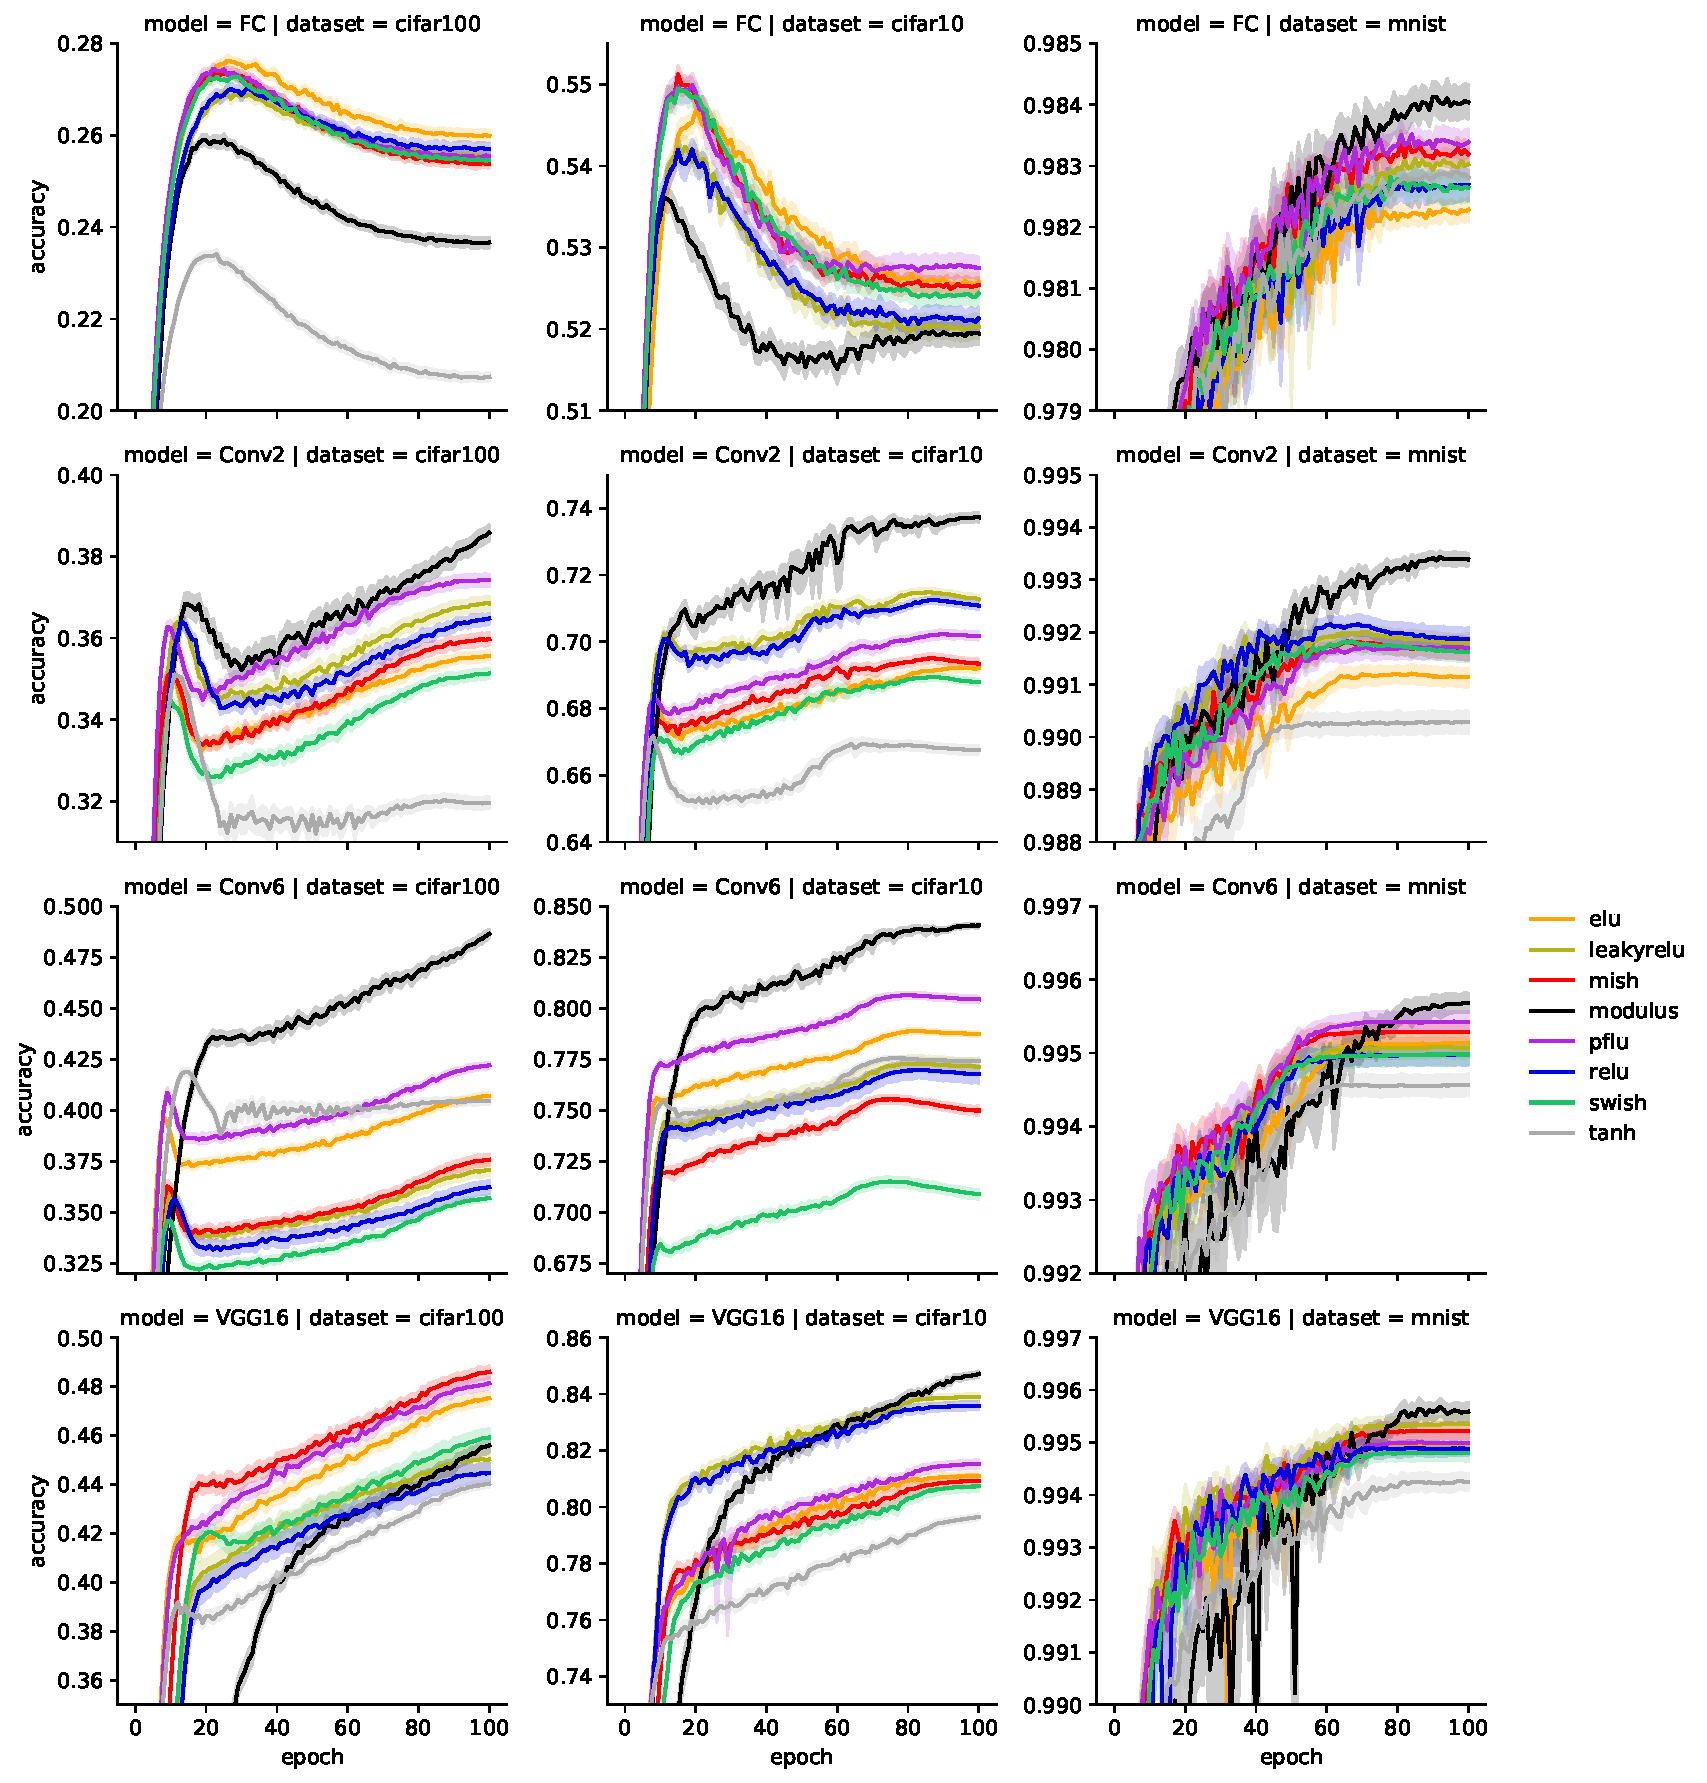
\includegraphics[width=1.0\linewidth]{modulus/images/training_curves}
	\caption{Training curves of all the trained models. Each line represents the average accuracy of 30 runs of a model. The shade beahind to each line shows the 95\% confidence interval around the mean. Notice that the scales in the y-axis are not shared to allow for better zoom in each figure, comparing the performance across models is not the objective of this study. Details like the shades are better viewed in a screen.}
	\label{fig:training_curves}
\end{figure}


The same experimental setup has been used across models, activations and datasets. All the networks have been trained for 100 epochs, and the best accuracy of each run has been recorded. Each run has been repeated 30 times with different random weight initializations. No \textit{dropout} \autocite{srivastava2014} nor \textit{batch normalization} \autocite{ioffe2015} have been used. \textit{Adam} \autocite{kingma14} has been used as optimizer, with a learning rate of $10^{-4}$, a \textit{gradual warmup} \autocite{gotmare2018} during the first 5 epochs starting from $10^{-5}$, and a \textit{cosine annealing} \autocite{loshchilov2017} with a target learning rate of $10^{-6}$ in the last epoch. The software versions used in all the chapter were: \textit{Python} 3.7.3, \textit{Pytorch} 1.7.1 and  \textit{TorchVision} 0.8.2. The code used in the experiments of this chapter can be found in the url included in the footnote \footnote{\url{https://github.com/ivallesp/abs}}.


\subsection{Results}
Table \ref{tab:modulus_results} summarizes the results of the classifiers for \textit{CIFAR10}, \textit{CIFAR100} and \textit{MNIST} datasets. As it can be seen from the tables, the \textit{modulus} activation function outperforms significantly the benchmark activations in 9 out of 12 experiments (4 architectures x 3 datasets). In 4 of these cases, the accuracy improvement is $3\%$ or higher, in relative terms. The \textit{SoftModulusT} approximation significantly outperforms the benchmark in 10 out of 12 experiments.

Figure \ref{fig:training_curves} shows the average training curves for the 12 experiments (the curves of the smooth approximations have been included in figure \ref{fig:training_curves_smooth} to compare them with the \textit{modulus}). As it can be noticed in several cases (e.g. \textit{CIFAR10-Conv2}, \textit{CIFAR10-Conv6}, \textit{CIFAR100-Conv6}), the accuracy of the networks with \textit{modulus} activation function keeps increasing at the 100th epoch while the benchmarks have already stabilized. That observation suggests that, if trained for longer, probably the accuracy would increase even more.


\begin{table}[hp!] \footnotesize  \setlength{\tabcolsep}{3pt}
	\caption{Accuracy comparison for the soft approximations of the \textit{modulus} function, compared with the original \textit{modulus} definition. The results are expressed as mean $\pm$ standard deviation across the 30 random initializations. The models with highest accuracy are highlighted in bold. A star is added to those cases where a \textit{SoftModulus} activation function achieved significantly higher results than the \textit{modulus}, with a significance level of $\alpha=0.05$.}
	\centering
	\begin{tabular}{rrcccc}
		\toprule
		 Dataset &   Activation &            FC             &           Conv2           &           Conv6           &           VGG16           \\ \midrule
		 CIFAR10 &      Modulus &     $53.97 \pm 0.24$      &     $73.93 \pm 0.42$      &     $84.22 \pm 0.29$      &     $84.86 \pm 0.32$      \\
		         & SoftModulusQ & $\mathbf{54.07 \pm 0.29}*$ &     $71.49 \pm 0.37$      &     $81.01 \pm 1.27$      &     $10.00 \pm 0.00$      \\
		         & SoftModulusT &     $54.04 \pm 0.24$      & $\mathbf{73.95 \pm 0.40}$ & $\mathbf{84.36 \pm 0.28}$ & $\mathbf{85.34 \pm 0.36}*$ \\ \midrule

		CIFAR100 &      Modulus &     $26.29 \pm 0.26$      &     $38.66 \pm 0.56$      & $\mathbf{48.73 \pm 0.62}$ &     $45.83 \pm 0.80$      \\
		         & SoftModulusQ &     $26.23 \pm 0.25$      &     $37.48 \pm 0.44$      &     $48.16 \pm 1.97$      &      $1.00 \pm 0.00$      \\
		         & SoftModulusT & $\mathbf{26.32 \pm 0.24}$ & $\mathbf{38.69 \pm 0.56}$ &     $48.63 \pm 0.83$      & $\mathbf{48.47 \pm 0.68}*$ \\ \midrule

		   MNIST &      Modulus &     $98.47 \pm 0.07$      &     $99.38 \pm 0.04$      &     $99.60 \pm 0.03$      & $\mathbf{99.63 \pm 0.04}$ \\
		         & SoftModulusQ & $\mathbf{98.51 \pm 0.06}*$ &     $99.37 \pm 0.03$      & $\mathbf{99.62 \pm 0.03}*$ &     $11.35 \pm 0.00$      \\
		         & SoftModulusT &     $98.47 \pm 0.06$      & $\mathbf{99.39 \pm 0.04}$ &     $99.61 \pm 0.03$      &     $99.62 \pm 0.03$      \\ \bottomrule
	\end{tabular}
	\label{tab:modulus_results_smooth}
\end{table}

\begin{figure}[h!]
	\centering
	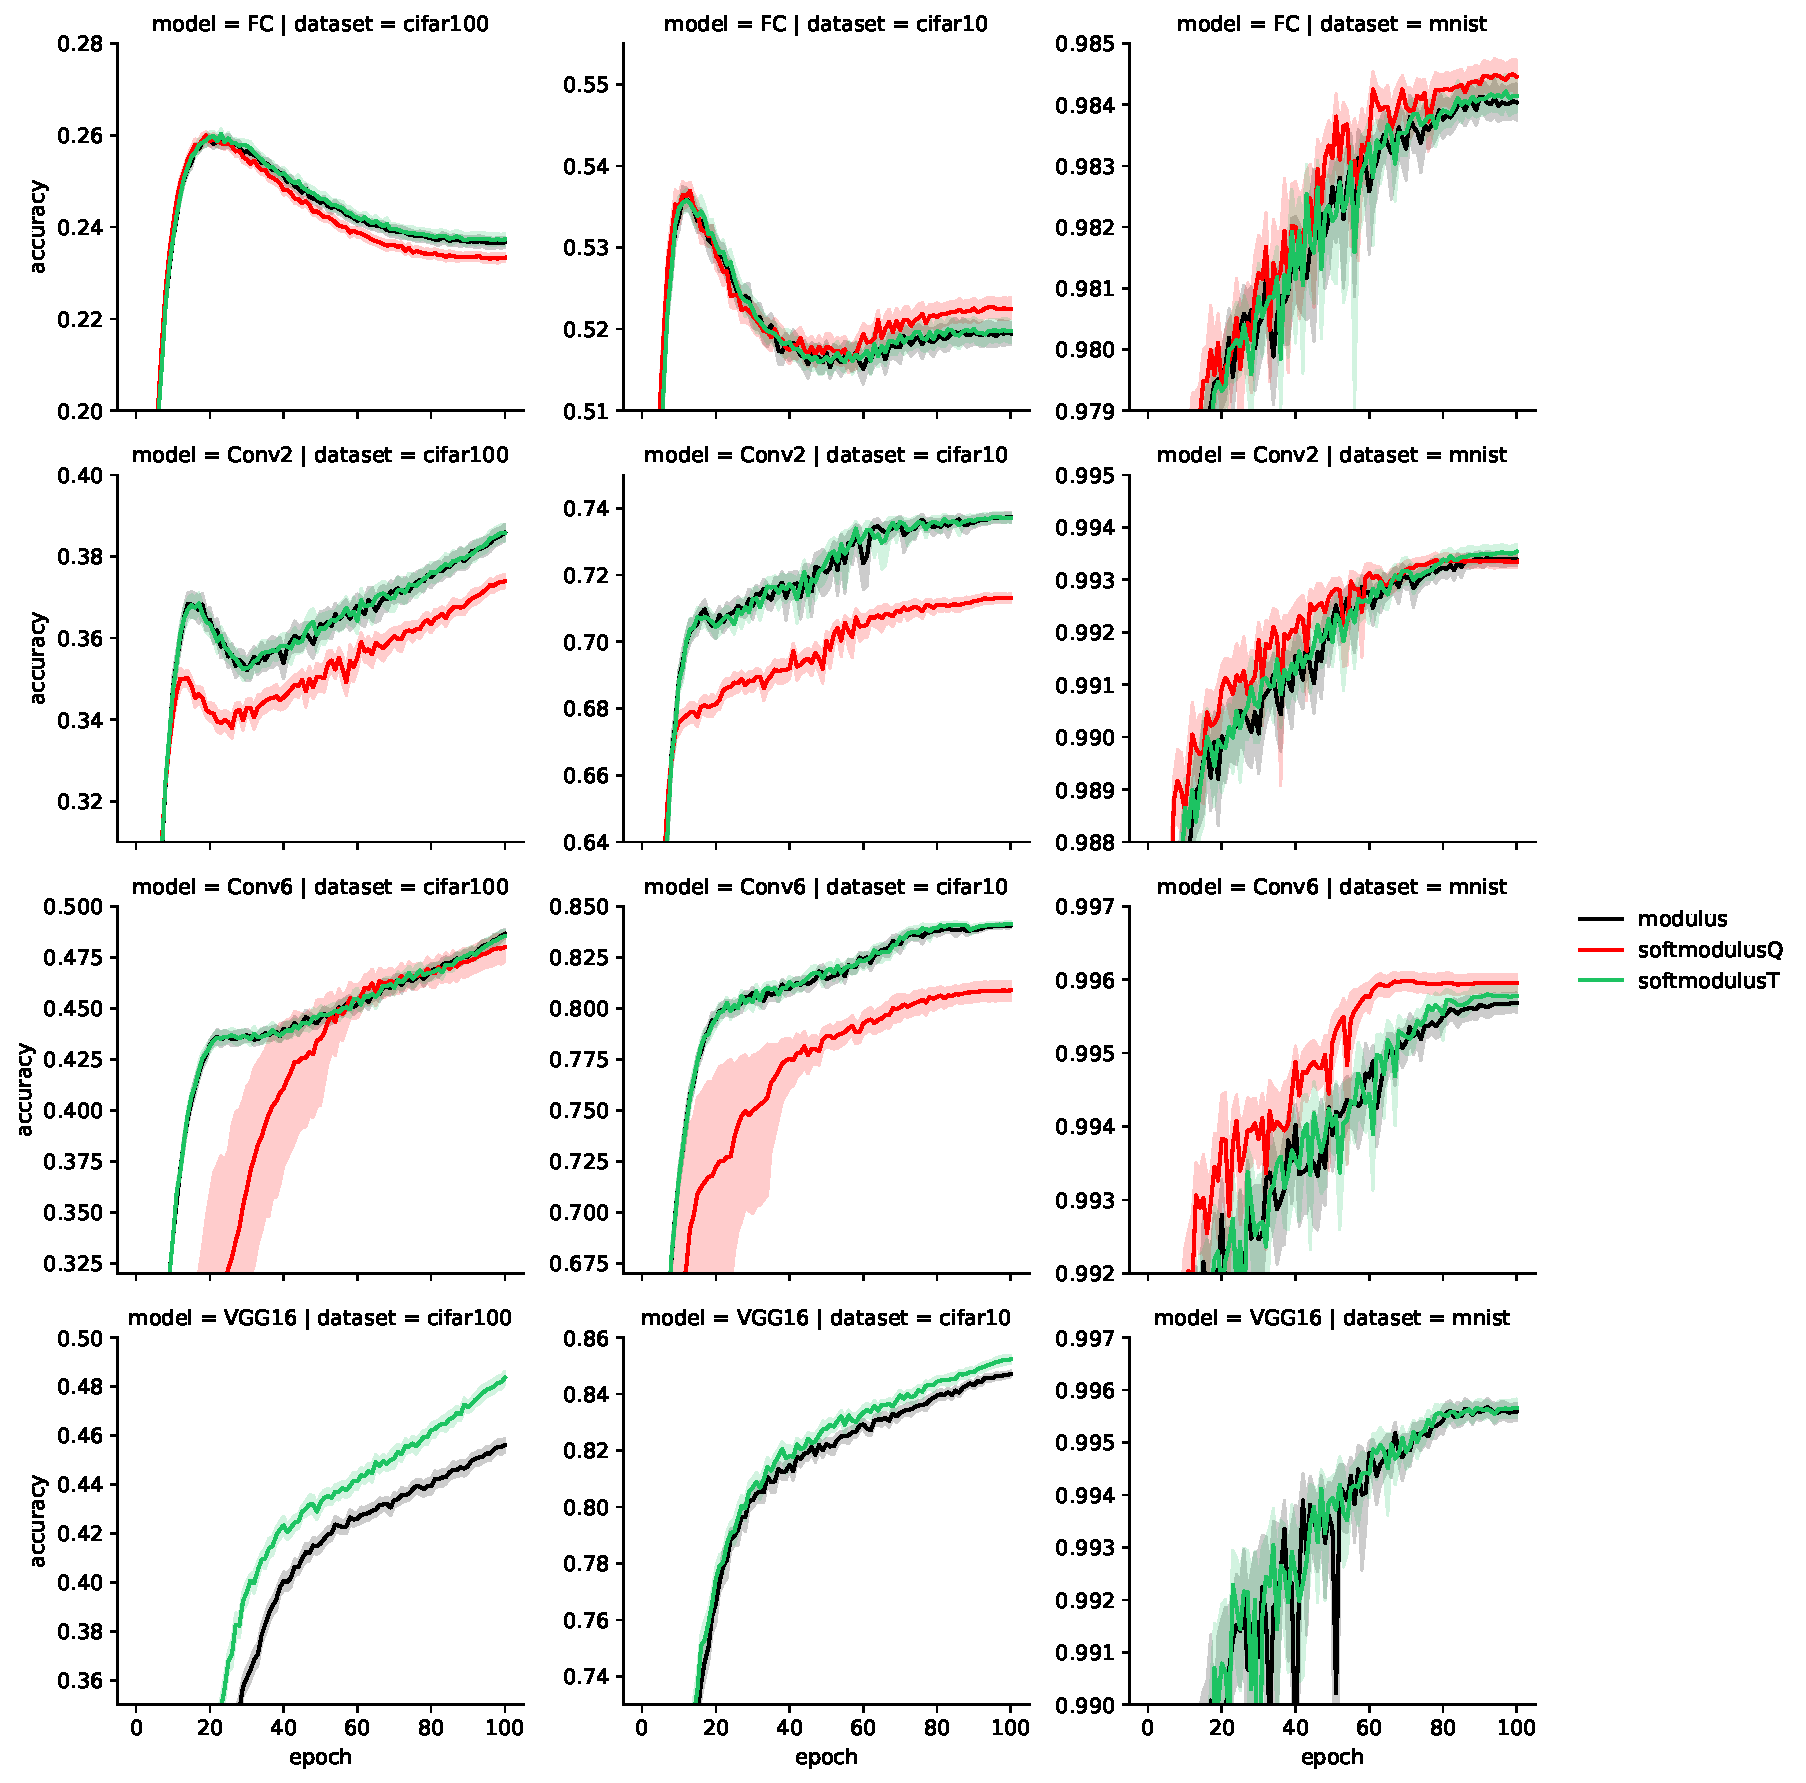
\includegraphics[width=1.0\linewidth]{modulus/images/training_curves_smooth}
	\caption{Training curves smooth approximations compared with the \textit{modulus}. Each line represents the average accuracy of 30 runs of a model. The shade behind to each line shows the 95\% confidence interval around the mean. Notice that the scales in the y-axis are not shared to allow for better zoom in each figure, comparing the performance across models is not the objective of this study. Details like the shades are better viewed in a screen.}
	\label{fig:training_curves_smooth}
\end{figure}

The results of the \textit{SoftModulus} approximations compared with the \textit{modulus} activation function are summarized in table \ref{tab:modulus_results_smooth}. Additionally, figure \ref{fig:training_curves_smooth} shows the training curves for the same activations. The \textit{SoftModulusQ} approximation achieved significantly better results than the original modulus in several cases (\textit{FC} model over \textit{CIFAR10} and \textit{MNIST} dataset, and \textit{Conv6} over \textit{MNIST} dataset); however it seems to be much more unstable: on VGG16, the gradients of the models with \textit{SoftModulusQ} activations vanish at the beginning of the training process due to the fact that the weights are initialized very close to zero and the gradients are too small, causing numerical issues. This problem may be solved tweaking the initialiation. However, the \textit{SoftModulusT} approximation seems to be on-par with the original \textit{modulus} in the majority of cases, while it performs significantly better for deep architectures like \textit{VGG16}. A plausible hypotyhesis explaining that observation is  that the difference between the two approximations is due to the width of the zero gradient region around $x=0$: wider regions lead to more training problems (see figure \ref{fig:activationssmooth}). The $\beta$ parameter in the hyperbolic tangent approximation allows for easily adjust this zero-gradient region. Different values of beta were informally tested concluding that for high values of $\beta$ (e.g. $\beta=1.0$) the model struggles to train due to numerical precision problems (small values of weights lead to tiny gradients). A value of $\beta=0.01$ seems to work well for all the tested experiments. Finally, the \textit{SoftModulusT} approximation achieves superior results than the original \textit{modulus} when used in the \textit{VGG16} architecture.




\section{Conclusions} \label{sec:modulus_conclusions}
This chapter provides evidences of how the proposed \textit{modulus} activation function outperforms the benchmark activation functions in 75\% of the experiments. The improvement achieved by the networks with this activation function is often significantly higher ($3\%$ or higher in 33.3$\%$ of the experiments conducted). Additionally, a smooth version of the \textit{modulus} activation function is proposed, even performs better than the first one, at a slightly higher computational cost.

The results of this chapter motivate exploring non-monotonic activation functions as alternatives to the classical choices.




